\documentclass{bioinfo}
\copyrightyear{2015}
\pubyear{2015}
\usepackage[normalem]{ulem}

\begin{document}
\firstpage{1}

\title[k-mer cardinality estimation]{Probabilistic cardinality estimation for fun and \sout{profit} SCIENCE!}
\author[Irber \textit{et~al}]{Luiz C. Irber Jr.\,$^{1,\footnote{to whom correspondence should be addressed}}$, C. Titus Brown\,$^{2,1,3}$ }
\address{$^{1}$Department of Computer Science and Engineering, Michigan State University, East Lansing 48823, \\
$^{2}$Department of Microbiology and Molecular Genetics, Michigan State University, East Lansing 48823, \\
$^{3}$Population Health and Reproduction, UC Davis, Davis 95616}

\history{Received on XXXXX; revised on XXXXX; accepted on XXXXX}

\editor{Associate Editor: XXXXXXX}

\maketitle

\begin{abstract} We present an open implementation of the
HyperLogLog cardinality estimation algorithm for counting fixed-length
subsequences of DNA (``k-mers'').
\section{Summary:}

\section{Availability and implementation:}

The HyperLogLog implementation is in C++ with a Python interface, and is distributed
as part of the khmer software package.
khmer is freely available from \href{https://github.com/ged-lab/khmer}{https://github.com/ged-lab/khmer} under a BSD License.
The features presented here are included in version 1.4 and later.

\section{Contact:} \href{irberlui@msu.edu}{irberlui@msu.edu}
\end{abstract}

%    Exact k-mer cardinality counting is too expensive/impractical, memory-wise.
%    Use cases for cardinality estimation on bioinformatics:
%        Bloom filter memory allocation
%            cite the SC14 paper
%            also QP's calculations
%    Probabilistic counting allows a tradeoff between accuracy and memory consumption
%    HLL is a fixed memory and pleasantly parallel data structure
%    Figures:
%        plot running time for different # of threads, with two bounds:
%            Just reading it from disk (I/O lower bound)
%            Running time for (diginorm? any operation using BF?), which should be the upper bound for performance. Using HLL is a tradeoff between running time and memory efficiency, but we don't want it increase runtime too much.
%        a comparison to other solutions (using sparsehash or python dicts) is not very informative (since HLL memory consumption will be constant). Maybe just a small table?
%    Implementation details:
%        why MurmurHash3?
%        OpenMP tasks

\section{Introduction}

DNA sequencing technologies have been increasing their data generation
capacity faster than Moore's Law for a decade or more, driving the
development of new computational analysis approaches.  A number of
probabilistic data structures and algorithms have been developed over
the last few year to deal with the rapidly increasing volume of data.
% bloom filter, melsted streaming, diginorm, etc.

Probabilistic data structures are useful when the cost for a exact
answer is prohibitive, but an approximate answer is acceptable.  The
approximation is usually attained through reproducible randomness
(hashing, for example) and average case analysis.  The main benefit of
probabilistic data structures is a tradeoff between space and
accuracy, since often a very small amount of memory can be used to obtain
crude results but better estimatives are reported as memory increases.
These data structures are usually specialized, performing one kind of
operation well but missing other functionality available on
generalized data structures.

Here we present an open implementation of the HyperLogLog cardinality
counting algorithm, specialized for fixed-length subsequences of DNA
strings, or ``k-mers''.  The HyperLogLog counter is a cardinality
estimation data structure with constant (and low) memory footprint,
based on hashing and probabilistic estimation.  (@Brief description.)
See Figure 2 for an example.

This functionality is useful for a variety of purposes, including
estimating the minimum required memory allocation for fixed-size data
structures such as Bloom filters and Count-Min Sketches (ref
\citep{pell2012scaling}, \citep{georganas2014parallel},
\citep{khmer-counting}) and estimating the memory required for
De Bruijn graph assemblers (cite Velvet).

%\citep{heule2013hyperloglog}

%\citep{flajolet2008hyperloglog}

%\citep{khmer2014}

\section{Methods}

We implemented HyperLogLog for k-mers on top of the khmer library.
khmer is a library and suite of command line tools for working with
DNA sequence.  It implements $k$-mer counting, read filtering and
graph traversal using probabilistic data structures that include Bloom
Filters and Count-Min Sketch.  Building on top of khmer leveraged the
existing infrastructure (read parsers, package installation, API
signatures and some k-mer hashing methods).

(Briefly describe HLL implementation, plus problem decomposition)

\subsection{The "add element" operation}

This operation involves the calculation of a hash value for the input,
some bitwise operations to determine special properties (longest run on 0-value bits, for example)
and a memory update to one position of the bit array.
This is the CPU-intensive part,
depending heavily on the hash function used.
We chose MurmurHash3 because it is one of the fastest non-cryptographic hash function available
and it has a reasonably uniform hash space distribution.
This is executed $len(read) - (k-1)$ times for each read on the dataset,
were $k$ is the desired $k$-mer size.

\subsection{HyperLogLog merge operation}

The merge operation is a elementwise max-reduction between two bit arrays.
Because the bit arrays are relatively small (about 128 KB) the merge operation is an excellent way to avoid resource sharing and synchronization during the update operations,
at the cost of instantiating additional temporary HyperLogLog structures.
Since their sizes are small,
this is a viable tradeoff.
This operation is not necessary when adding elements in parallel and can be executed
optimally after all elements were consumed (i.e. once at the end).

\subsection{Problem decomposition}

One way to divide the problem is by instantiating multiple HLL counters
and distributing reads between them while iterating over the data.
After all the reads are consumed the counters are merged and the final
counter can be used for cardinality estimation.

We chose a shared memory implementation for this problem
decomposition, since only a small amount of memory is needed and this
is also the architecture most potential users have available for use.
OpenMP was chosen because it doesn't demand code changes (meaning the
program will still work if OpenMP is not available, although slower).
This is also important because it is not available currently (January
2015) on the default OSX compiler (clang), but as soon clang
implements OpenMP support it will work for khmer users.  This would be
harder to implement with MPI, the other common parallelization
mechanism.

The only shared resource during updates is the bit array.  In order to
avoid any synchronization instead of having one HyperLogLog shared
between threads (and so a critical section or atomic update of the bit
array position) We opted for creating one HyperLogLog data structure
for each thread, so that no resources need to be shared.

OpenMP tasks maps well to this decomposition: one thread (using a
single pragma) get reads from the read parser and for each read a task
is spawned, using firstprivate(read) to guarantee the read won't be
overwritten.  The task thread does the ``add element'' operation in
the counter assigned to its thread ID.  After all reads are parsed and
the tasks finish one thread does the merge operation over all
counters.

Since the sequential HyperLogLog implementation is CPU-bound (limited by hashing),
optimized input reading is not a priority.

\section{Discussion}

%Items for discussion:
%
%\begin{itemize}
%\item It's fast; estimate per mn reads, linear evaluation, including startup.

%\item Further speedups are unlikely: we're IO bound currently.

Running with only one CPU is suboptimal because the problem can be easily parallelized,

and hashing is CPU-bound.

For comparison we ran a simple benchmark using the same input infrastructure,
but without performing any kind of processing to check what is the I/O lower bound.
This baseline can be used to verify how many threads are needed before I/O becomes the bottleneck.

Figure \ref{fig:02} shows $t=32$ threads are needed to saturate I/O.

%\item Estimate practical memory usage (Python included).


Memory consumption increases proportionally to the number of threads
used, since one HyperLogLog is instantiated for each thread.  The
increase in memory consumption is not a practical problem because each
HyperLogLog counter is small: Figure \ref{fig:03} shows the maximum
resident memory for pure I/O is about 25 MB, (...)  At the end of
input processing this memory can be released by merging all
HyperLogLog holding the partial counts into one containing the final
result.

Another memory overhead associated with increasing the number of
threads is the memory OpenMP allocations for its task queue, which
depend on the compilers' implementation.  % TODO: verify if the
memory allocated by OpenMP can be changed!  This is not so drastic
because the thread doing input parsing can switch to sequence
processing if the queue is full, and in I/O saturation conditions the
queue will be almost empty all the time.


%\end{itemize}


We implemented parallelization in shared memory using OpenMP.
Shared memory parallelization is useful because the most time consuming
step is calculating the hash and this doesn't share state among other calculations.
The critical operation is updating the bit arrays,
which is fast and just modify a small amount of memory.

The target architecture is multicore CPUs.
The primary users of khmer are biologists and one of the project goals is easy installation and a low cognitive barrier for new users.
Compiling in a consistent way for Xeon Phi or GPUs is non-trivial in most systems,
and even OpenMP is not supported in some popular platforms (OSX + clang, for example).
Nonetheless,
adapting the code to use either Xeon Phi or GPUs could lead to even better results,
since the hashing process is mostly CPU-bound.

We used two different datasets during development,
one being a subset 3 orders of magnitude smaller than the other:

Gallus\_3.longest25.fasta

  - 149,943,923 bp
  - 44,336 seqs
  - 3,382.0 average length
  - 144 MB

Despite being smaller,
the average length of each sequence is about the same for both datasets.
I used the partial dataset just to make quick tests

The true cardinality of the complete dataset for $k=32$ is 129,196,601.
This is the timing data for the complete dataset (all tests with k=32):

Speedup times are close to linear,
which is best seem on Figure 3.
We can also notice the estimation is within error bounds,
being smaller than 1%.

For stress testing I used a larger dataset.
Although it's 4 times smaller than the one I proposed to use,
it is a typical dataset found by users.

Chicken\_10Kb20Kb\_40X\_Filtered\_Subreads.fastq

  - 43,076,933,303 bp
  - 9,006,923 seqs
  - 4,782.6 average length
  - 81 GB

Using the Python API, with 16 threads and k = 32,
the running time is close to what is expected when extrapolating the
results on smaller datasets,
(about 36 minutes).

%``` bash
%  $ time python unique_kmers.py Chicken_10Kb20Kb_40X_Filtered_Subreads.fastq 32
%  unique k-mers: 41,954,729,591
%  real    35m2.600s user    326m27.120s sys     2m53.487s
%```

\section{Conclusion}

\section*{Acknowledgement}

\paragraph{Funding\textcolon} This work was supported by FUNDING-AGENCY [ GRANT-NUMBER ].

\bibliographystyle{natbib}
%\bibliographystyle{achemnat}
%\bibliographystyle{plainnat}
%\bibliographystyle{abbrv}
%\bibliographystyle{bioinformatics}
%
%\bibliographystyle{plain}
%
\bibliography{2014-hll}


\begin{figure*}[!tpb]%figure2
\centerline{\includegraphics[width=\textwidth]{figures/io_bound.png}}
\caption{Walltime and lower bound(I/O)}\label{fig:walltime}
\end{figure*}

\begin{figure*}[!tpb]%figure3
\centerline{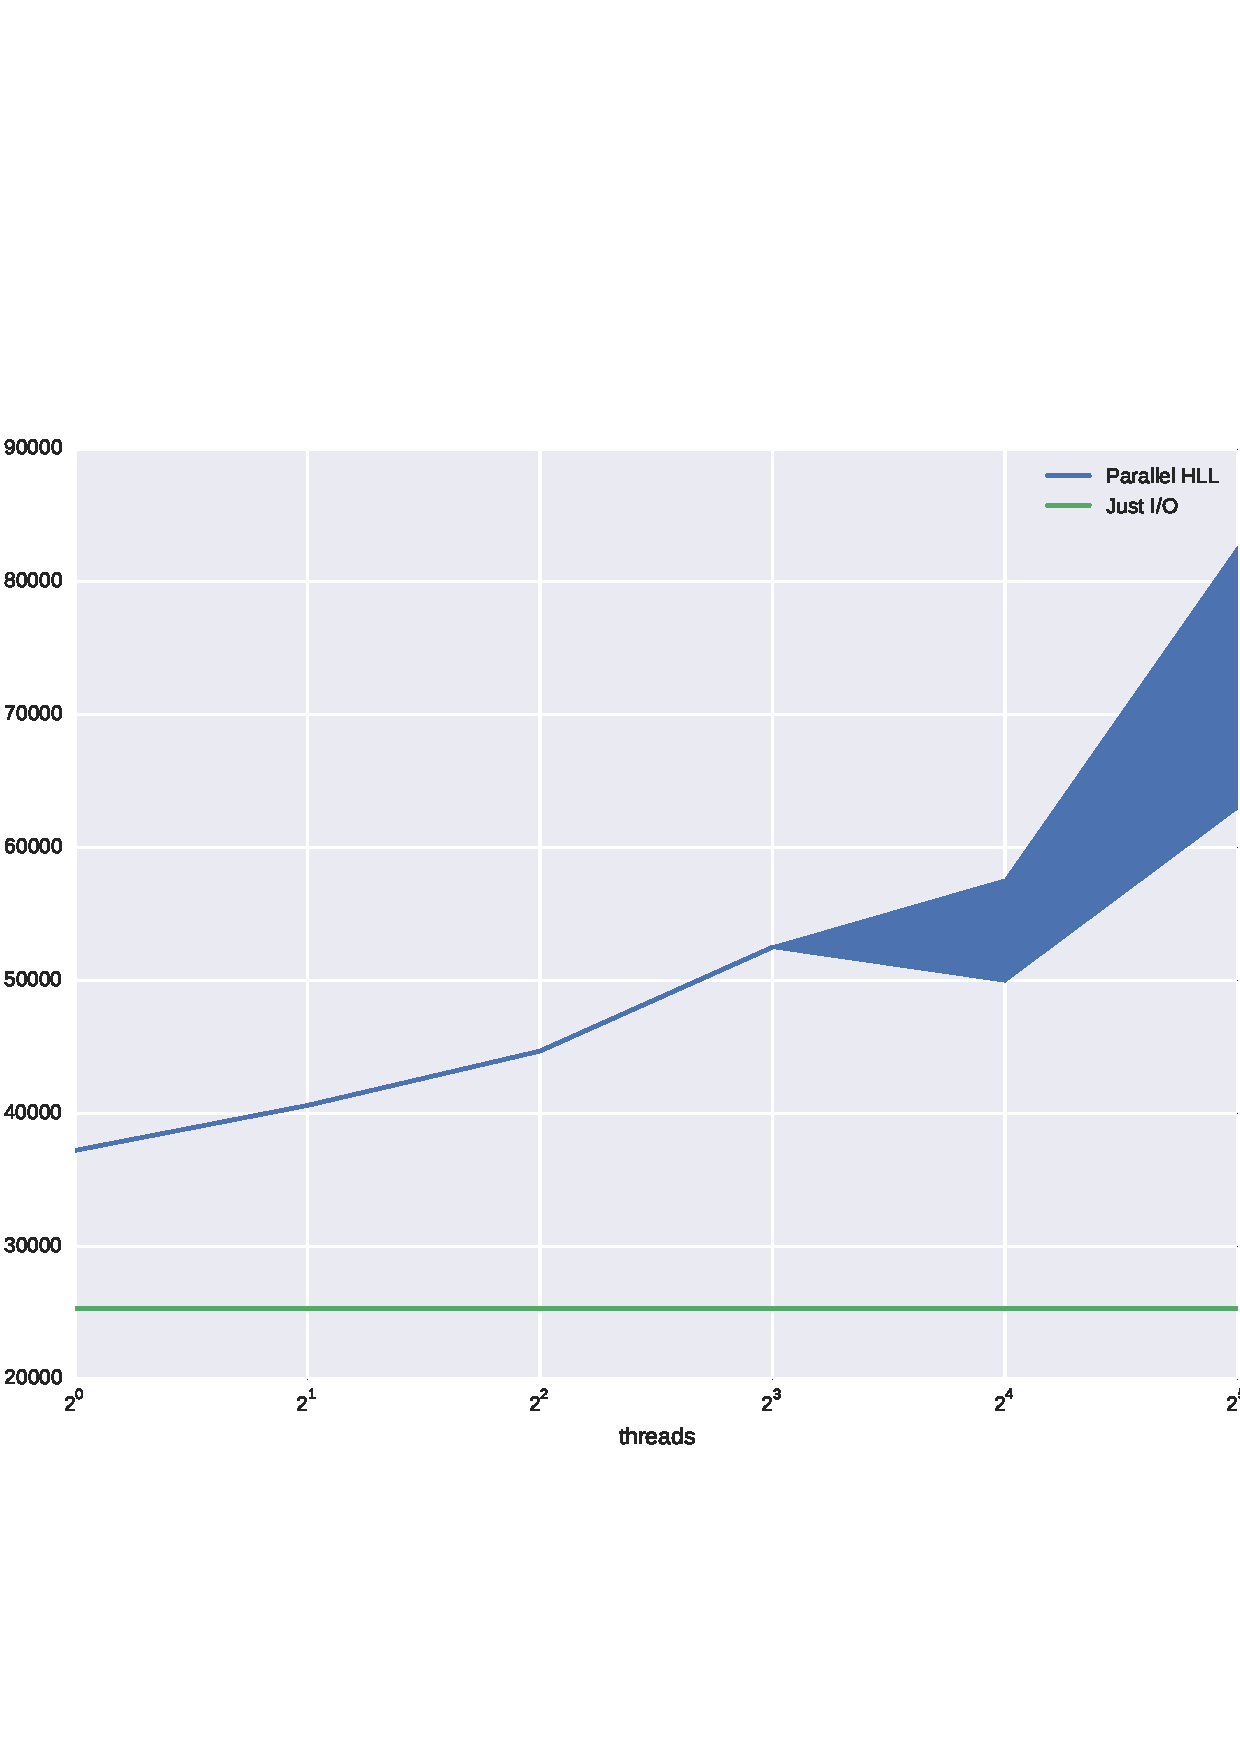
\includegraphics[width=\textwidth]{figures/mem_consumption.png}}
\caption{Memory consumption}\label{fig:mem}
\end{figure*}


\end{document}
